%%%%%%%%%%%%%%%%%%%%%%%%%%%%%%%%%%%%%%%%%
% Beamer Presentation
% LaTeX Template
% Version 1.0 (10/11/12)
%
% This template has been downloaded from:
% http://www.LaTeXTemplates.com
%
% License:
% CC BY-NC-SA 3.0 (http://creativecommons.org/licenses/by-nc-sa/3.0/)
%
%%%%%%%%%%%%%%%%%%%%%%%%%%%%%%%%%%%%%%%%%

%----------------------------------------------------------------------------------------
%	PACKAGES AND THEMES
%----------------------------------------------------------------------------------------

\documentclass{beamer}

\mode<presentation> {

  % The Beamer class comes with a number of default slide themes
  % which change the colors and layouts of slides. Below this is a list
  % of all the themes, uncomment each in turn to see what they look like.

  % \usetheme{default}
  % \usetheme{AnnArbor}
  % \usetheme{Antibes}
  % \usetheme{Bergen}
  % \usetheme{Berkeley}
  % \usetheme{Berlin}
  % \usetheme{Boadilla} *
  % \usetheme{CambridgeUS}
  % \usetheme{Copenhagen}
  % \usetheme{Darmstadt}
  % \usetheme{Dresden}
  \usetheme{Frankfurt}
  % \usetheme{Goettingen}
  % \usetheme{Hannover}
  % \usetheme{Ilmenau}
  % \usetheme{JuanLesPins}
  % \usetheme{Luebeck}
  % \usetheme{Madrid}
  % \usetheme{Malmoe}
  % \usetheme{Marburg}
  % \usetheme{Montpellier}
  % \usetheme{PaloAlto}
  % \usetheme{Pittsburgh}
  % \usetheme{Rochester}
  % \usetheme{Singapore}
  % \usetheme{Szeged}
  % \usetheme{Warsaw}

  % As well as themes, the Beamer class has a number of color themes
  % for any slide theme. Uncomment each of these in turn to see how it
  % changes the colors of your current slide theme.

  % \usecolortheme{albatross}
  % \usecolortheme{beaver}
  % \usecolortheme{beetle}
  % \usecolortheme{crane}
  % \usecolortheme{dolphin}*
  % \usecolortheme{dove}
  % \usecolortheme{fly}
  % \usecolortheme{lily}
  % \usecolortheme{orchid}
  % \usecolortheme{rose}
  % \usecolortheme{seagull}
  % \usecolortheme{seahorse}
  % \usecolortheme{whale}
  % \usecolortheme{wolverine}

  %\setbeamertemplate{footline} % To remove the footer line in all slides uncomment this line
  % \setbeamertemplate{footline}[page number] % To replace the footer line in all slides with a simple slide count uncomment this line

  % \setbeamertemplate{navigation symbols}{} % To remove the navigation symbols from the bottom of all slides uncomment this line
}

\usepackage{graphicx} % Allows including images
\usepackage{booktabs} % Allows the use of \toprule, \midrule and \bottomrule in tables


\usepackage{adjustbox}

\newcommand\floor[1]{\lfloor#1\rfloor}
\usepackage{array}
\newcolumntype{L}[1]{>{\raggedright\let\newline\\\arraybackslash\hspace{0pt}}m{#1}}
\newcolumntype{C}[1]{>{\centering\let\newline\\\arraybackslash\hspace{0pt}}m{#1}}
\newcolumntype{R}[1]{>{\raggedleft\let\newline\\\arraybackslash\hspace{0pt}}m{#1}}
\usepackage{makecell}

%----------------------------------------------------------------
%
% Tikz
%
%----------------------------------------------------------------
\usepackage{tikz}
\usetikzlibrary{shapes.geometric,backgrounds,calc}
\tikzset{
    basic box/.style = {
        shape = rectangle,
        align = center,
        draw  = #1,
        fill  = #1!25,
        minimum width=4.4cm,
        minimum height=1cm,
        rounded corners
    },
    guest os/.style = {
        shape = rectangle,
        align = center,
        draw  = #1,
        fill  = #1!25,
        minimum width=2.15cm,
        minimum height=1cm,
        rounded corners
    },
    app guest os/.style = {
        shape = rectangle,
        align = center,
        draw  = #1,
        fill  = #1!25,
        minimum width=2.15cm,
        minimum height=1cm,
        rounded corners
    }
}
\usepackage{pgfplots}

%----------------------------------------------------------------------------------------
%	TITLE PAGE
%----------------------------------------------------------------------------------------

\title[Software-Based TG using Docker]{An Evaluation of Software-Based\\Traffic Generators using Docker} % The short title appears at the bottom of every slide, the full title is only on the title page

\author{Sai Man Wong} % Your name
\institute[KTH] % Your institution as it will appear on the bottom of every slide, may be shorthand to save space
{
  KTH Royal Institute of Technology\\ % Your institution for the title page
  School of Computer Science and Communication\\
  \medskip
  \textit{smwong[a]kth.se} % Your email address
}
\date{\today} % Date, can be changed to a custom date

\begin{document}

\begin{frame}
  \titlepage % Print the title page as the first slide
\end{frame}

\section{Why...}
\subsection{}
\begin{frame}
  \frametitle{Why...}
  \begin{itemize}
    \item ... software-based traffic generators?
    \item ... this thesis work?
  \end{itemize}
\end{frame}

% TOC
\section{}
\begin{frame}
  \frametitle{Overview} % Table of contents slide, comment this block out to remove it
  \tableofcontents % Throughout your presentation, if you choose to use \section{} and \subsection{} commands, these will automatically be printed on this slide as an overview of your presentation
\end{frame}

%----------------------------------------------------------------------------------------
%	PRESENTATION SLIDES
%----------------------------------------------------------------------------------------

%----------------------------------------------------------------------------------------
%	Software-Based Traffic Generator
%----------------------------------------------------------------------------------------
\section{Software-Based Traffic Generator}
\subsection{}
\begin{frame}
  \frametitle{Software-Based Traffic Generator}
  \begin{columns}[c] % The "c" option specifies centered vertical alignment while the "t" option is used for top vertical alignment
    \column{.5\textwidth} % Left column and width
    \textbf{Hardware-Based \\ Traffic Generator}
    \begin{itemize}
      \item Expensive
      \item Rigid
      \item Accurate
    \end{itemize}

    \column{.5\textwidth} % Right column and width
    \textbf{Software-Based \\ Traffic Generator}
    \begin{itemize}
      \item Cheap
      \item Flexible
      \item Inaccurate
    \end{itemize}
  \end{columns}
\end{frame}

\begin{frame}
  \frametitle{Types/Metrics}
  \begin{block}{(*) User Space}
    Default network stack, \\
    e.g., Iperf, Mausezahn, Ostinato and Tcpdump
  \end{block}

  \begin{block}{Kernel Space}
    Loadable Kernel Module, \\
    e.g., Brute and Pktgen
  \end{block}

  \begin{block}{External Framework}
    Circumvent the default network stack, \\
    e.g., MoonGen and TRex
  \end{block}
\end{frame}

\begin{frame}
  \frametitle{Types/Metrics contd.}
  \begin{table}[ht!]
    \scriptsize
    \caption{Summary of Traffic Generators Types}
    \label{types}
    \begin{adjustbox}{center}
        \renewcommand*\arraystretch{1.0}\begin{tabular}{| L{4cm} | L{7cm} |}
            \hline
            \textbf{Replay Engines} & Replay network traffic back to specified NIC from a file which contains prerecorded traffic, usually a pcap-file.
            \\ \hline
            \textbf{(*) Maximum Throughput Generators} & Generate maximum of network traffic with the purpose to test overall network performance, for example, over a link.
            \\ \hline
            \textbf{Model-Based Generators} & Generate network traffic based on stochastic models.
            \\ \hline
            \textbf{High-Level and Auto-Configurable Generators} & Generate traffic from realistic network models and change the parameters accordingly.
            \\ \hline
            \textbf{Special Scenario Generators} & Generate network traffic with a specific characteristic, for example, video streaming traffic.
            \\ \hline \hline
            \textbf{Application-level Traffic generators} & Generate network traffic of network applications, for example, the traffic behavior between servers and clients.
            \\ \hline
            \textbf{Flow-Level Traffic generators} & Generate packets in a particular order that resembles a particular characteristic from source to destination, for example, Internet traffic.
            \\ \hline
            \textbf{(*) Packet-Level Traffic Generators} & Generate and craft packets, usually, from layer 2 and up to 7.
            \\ \hline
        \end{tabular}
    \end{adjustbox}
\end{table}

\end{frame}

%----------------------------------------------------------------------------------------
%	Virtualization
%----------------------------------------------------------------------------------------
\section{Virtualization}
\subsection{}
\begin{frame}
  \frametitle{Virtualization}
  \begin{figure}[h!]
  \begin{adjustbox}{width=1\textwidth, center}
    \renewcommand*\arraystretch{1.5}
    \centering
    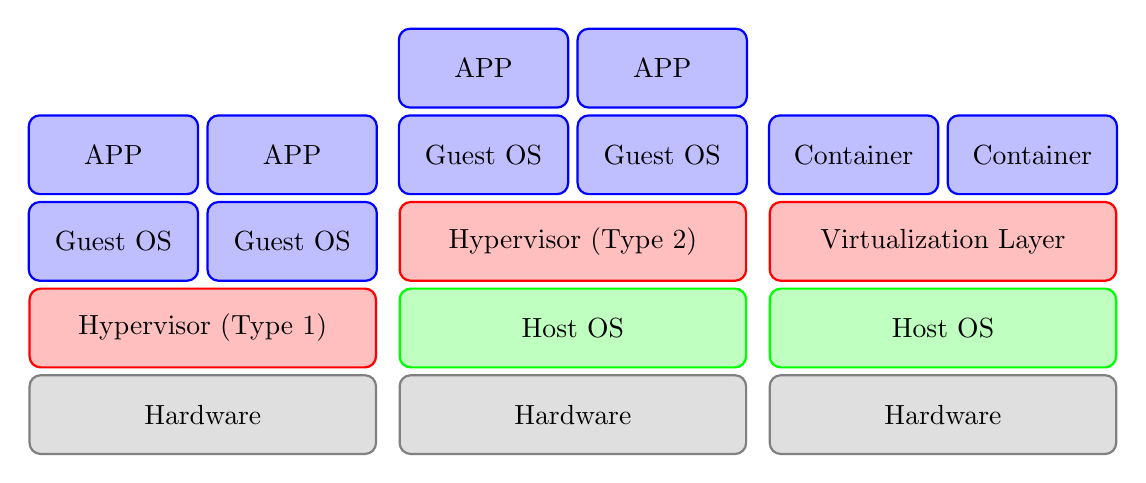
\begin{tikzpicture}[node distance = 1.2cm, thick, nodes = {align = center}, >=latex]
      \node at (0,0) [basic box = gray] {Hardware};
      \node at (0,1.1) [basic box = red] {Hypervisor (Type 1)};
      \node at (-1.135, 2*1.1) [guest os = blue] {Guest OS};
      \node at (1.135, 2*1.1) [guest os = blue] {Guest OS};
      \node at (-1.135, 3*1.1) [guest os = blue] {APP};
      \node at (+1.135, 3*1.1) [guest os = blue] {APP};

      \node at (4.7, 0) [basic box = gray] {Hardware};
      \node at (4.7, 1.1) [basic box = green] {Host OS};
      \node at (4.7,2*1.1) [basic box = red] {Hypervisor (Type 2)};
      \node at (4.7-1.135, 3*1.1) [guest os = blue] {Guest OS};
      \node at (4.7+1.135, 3*1.1) [guest os = blue] {Guest OS};
      \node at (4.7-1.135, 4*1.1) [guest os = blue] {APP};
      \node at (4.7+1.135, 4*1.1) [guest os = blue] {APP};

      \node at (2*4.7, 0) [basic box = gray] {Hardware};
      \node at (2*4.7, 1.1) [basic box = green] {Host OS};
      \node at (2*4.7, 2*1.1) [basic box = red] {Virtualization Layer};
      \node at (9.4-1.135, 3*1.1) [guest os = blue] {Container};
      \node at (9.4+1.135, 3*1.1) [guest os = blue] {Container};
    \end{tikzpicture}
  \end{adjustbox}
  \caption{Hypervisor-Based (Type 1 and 2) and Container-Based Virtualization}
  \label{fig:virtualization}
\end{figure}

\end{frame}

\begin{frame}
  \frametitle{Docker Architecture}
  \begin{itemize}
    \item cgroups ``limits how much you can use''
    \item namespaces ``limits what you can see (and therefore use)''
  \end{itemize}
  \begin{figure}[h!]
    \centering
    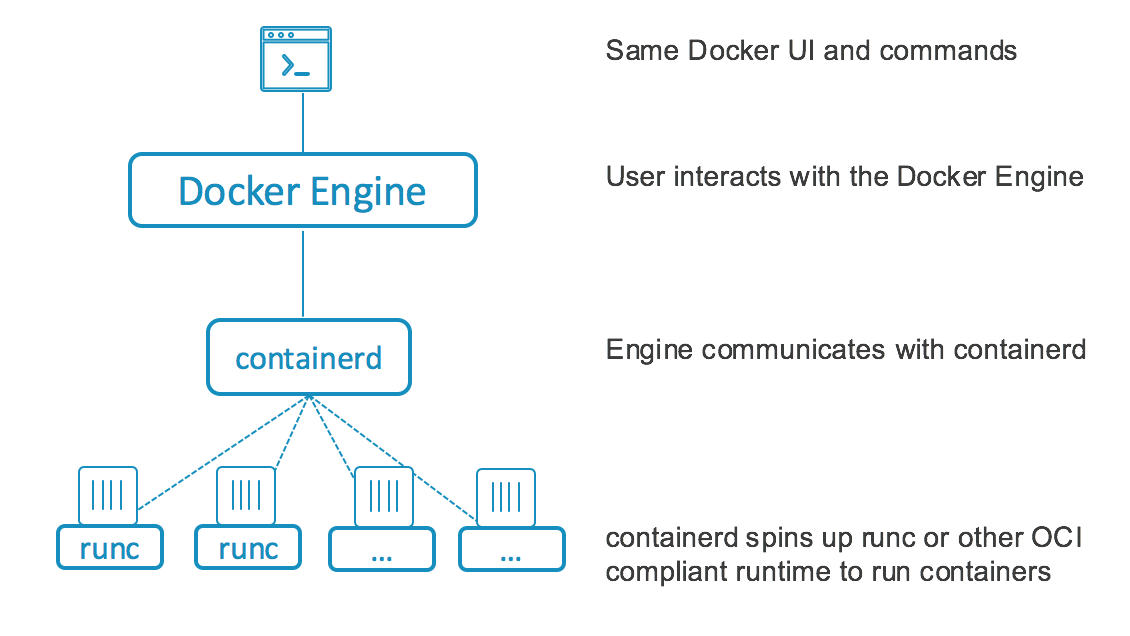
\includegraphics[width=8cm]{../tex/figure/dockerarchblog}
    \caption{Overview of Docker Architecture}
    \label{fig:arch}
  \end{figure}
\end{frame}

\section{Experiments}
\subsection{}
\begin{frame}
  \frametitle{Experiments}
  \begin{columns}[c] % The "c" option specifies centered vertical alignment while the "t" option is used for top vertical alignment
    \column{.5\textwidth} % Left column and width
    \textbf{Tools}
    \begin{itemize}
      \item Iperf \\ (infinite packets)
      \item Mausezahn \\ (infinite packets)
      \item Ostinato \\ (infinite burst packets)
      \item Tcpdump \& Capinfos \\ (capture and analysis)
    \end{itemize}

    \column{.5\textwidth} % Right column and width
    \textbf{Data Collection}
    \begin{itemize}
      \item Source to sink
      \item UDP traffic \\
        64 -- 4096 bytes packet size
      \item 10 seconds x 100 iterations
    \end{itemize}
  \end{columns}
\end{frame}

\subsection{Physical Environment}
\begin{frame}
  \frametitle{Physical Environment}
  \begin{figure}[h!]
    \centering
    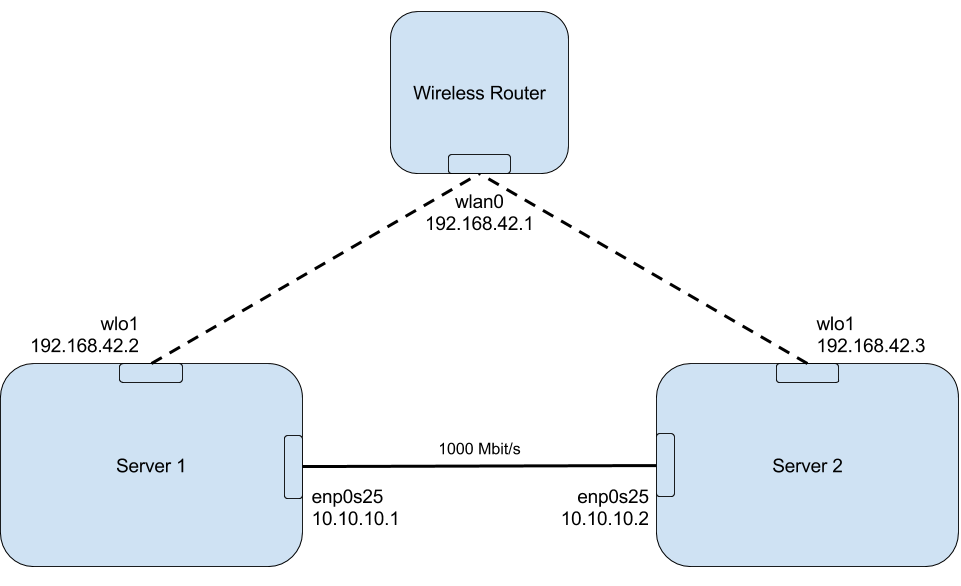
\includegraphics[width=10.5cm]{../tex/figure/labenv}
    \caption{Overview of Physical Lab}
    \label{fig:labenv}
  \end{figure}
\end{frame}

\begin{frame}
  \frametitle{Physical Environment: Results}
  \begin{columns}[c] % The "c" option specifies centered vertical alignment while the "t" option is used for top vertical alignment
    \column{.70\textwidth} % Left column and width
    \begin{figure}[h!]
    \begin{adjustbox}{width=1\textwidth, center}
        \renewcommand*\arraystretch{1.5}
        \begin{tikzpicture}
            \begin{axis}[
                title={},
                legend style={font=\scriptsize},
                x label style = {text height = 0.7cm},
                xlabel={Packet Size in Bytes},
                ylabel={Throughput in Megabit Per Second},
                xmin=0, xmax=4096,
                ymin=0, ymax=1100,
                xtick={0, 1000, 2000, 3000, 4000, 5000},
                ytick={0, 200, 400, 600, 800, 1000},
                legend pos=south east,
                ymajorgrids=true,
                grid style=dashed,
                height=11cm,
                width=20cm,
                /pgf/number format/.cd,
                1000 sep={}
                ]

                \addplot [color=black, mark=o]
                plot [error bars/.cd, y dir = both, y explicit]
                table[y error index=2]{../tex/plot/host_theoretical.dat};

                \addplot [color=blue, mark=o]
                plot [error bars/.cd, y dir = both, y explicit]
                table[y error index=2]{../tex/plot/host_ostinato.dat};

                \addplot [style=thick, color=red, mark=o]
                plot [error bars/.cd, y dir = both, y explicit]
                table[y error index=2]{../tex/plot/host_mausezahn.dat};

                \addplot [color=green, mark=o]
                plot [error bars/.cd, y dir = both, y explicit]
                table[y error index=2]{../tex/plot/host_iperf.dat};

                \legend{Theoretical, Ostinato, Mausezahn, Iperf}

            \end{axis}
        \end{tikzpicture}
    \end{adjustbox}
    \caption{Throughput Graph Summary in Physical Environment}
    \label{fig:experiment_host}
\end{figure}

    \column{.30\textwidth} % Right column and width
    \begin{itemize}
      \item Ostinato 984.61 Mbps \\@ 4096
      \item Iperf \& Mausezahn 965 Mbps \\@ 3072
      \item 12\% and 75\% below limit @ 64 -- 512
    \end{itemize}
  \end{columns}
\end{frame}

\subsection{Virtual Environment}
\begin{frame}
  \frametitle{Virtual Environment}
  \begin{figure}[h!]
    \centering
    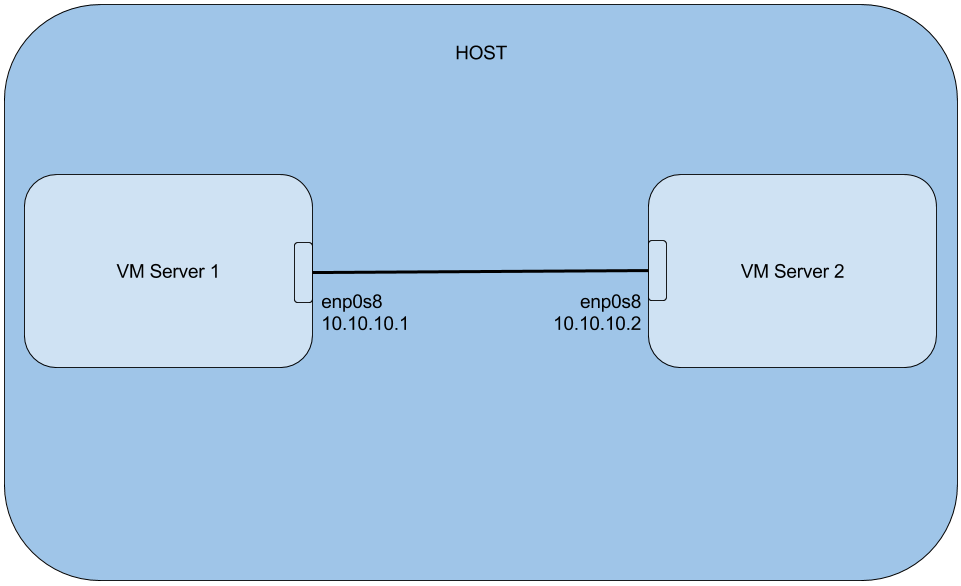
\includegraphics[width=10.5cm]{../tex/figure/vmenv}
    \caption{Overview of Virtual Lab}
    \label{fig:vmenv}
  \end{figure}
\end{frame}

\begin{frame}
  \frametitle{Virtual Environment: Results}
  \begin{columns}[c] % The "c" option specifies centered vertical alignment while the "t" option is used for top vertical alignment
    \column{.70\textwidth} % Left column and width
    \begin{figure}[h!]
    \begin{adjustbox}{width=1\textwidth, center}
        \renewcommand*\arraystretch{1.5}
        \begin{tikzpicture}
            \begin{axis}[
                title={},
                legend style={font=\scriptsize},
                x label style = {text height = 0.7cm},
                xlabel={Packet Size in Bytes},
                ylabel={Throughput in Megabit Per Second},
                xmin=0, xmax=4096,
                ymin=0, ymax=2100,
                xtick={0, 1000, 2000, 3000, 4000, 5000},
                ytick={0, 200, 400, 600, 800, 1000, 1200, 1400, 1600, 1800, 2000, 2200},
                legend pos=south east,
                ymajorgrids=true,
                grid style=dashed,
                height=11cm,
                width=20cm,
                /pgf/number format/.cd,
                1000 sep={}
                ]

                \addplot [color=black, mark=o]
                plot [error bars/.cd, y dir = both, y explicit]
                table[y error index=2]{../tex/plot/vm_theoretical.dat};

                \addplot [color=blue, mark=o]
                plot [error bars/.cd, y dir = both, y explicit]
                table[y error index=2]{../tex/plot/vm_ostinato.dat};

                \addplot [color=red, mark=o]
                plot [error bars/.cd, y dir = both, y explicit]
                table[y error index=2]{../tex/plot/vm_mausezahn.dat};

                \addplot [color=green, mark=o]
                plot [error bars/.cd, y dir = both, y explicit]
                table[y error index=2]{../tex/plot/vm_iperf.dat};

                \legend{Theoretical, Ostinato, Mausezahn, Iperf}

            \end{axis}
        \end{tikzpicture}
    \end{adjustbox}
    \caption{Throughput Graph Summary in Virtual Environment}
    \label{fig:experiment_vm}
\end{figure}

    \column{.30\textwidth} % Right column and width
    \begin{enumerate}
      \item Around 2000 Mbps
      \item ``internal-networking mode''
      \item CPU depended
    \end{enumerate}
  \end{columns}
\end{frame}

\subsection{Recommendation \& Conclusion}
\begin{frame}
  \frametitle{Recommendation \& Conclusion}
  \begin{columns}[c] % The "c" option specifies centered vertical alignment while the "t" option is used for top vertical alignment
    \column{.50\textwidth} % Left column and width
    \textbf{Recommendation}
    \begin{enumerate}
      \item Craft arbitrary packets: Mausezahn and Ostinato
      \item Automation: \\Ostinato
      \item Bandwidth test: \\Iperf
    \end{enumerate}
    \column{.50\textwidth} % Right column and width
    \textbf{Conclusion}
    \begin{enumerate}
      \item Smaller end-to-end system tests
      \item Suitable with container technology for automation capabilities and reproducibility
    \end{enumerate}
  \end{columns}
\end{frame}

\section{Demo}
\subsection{Run a container (CLI)}
\begin{frame}[fragile]
  \frametitle{Run a container (CLI)}
  \begin{example}[\texttt{test.py}]
    \begin{verbatim}
import time
while True:
    print("hello there")
    time.sleep(3)
    \end{verbatim}
  \end{example}

  \texttt{
    \$ docker run --rm -it \\\qquad
    --name demo1 \\\qquad
    -v \$PWD/test.py:/test.py \\\qquad
    python:latest python test.py
  }
\end{frame}
\subsection{Run a container (Dockerfile)}
\begin{frame}[fragile]
  \frametitle{Run a container (Dockerfile)}
  \begin{example}[\texttt{Dockerfile}]
    \begin{verbatim}
FROM python

COPY test.py test.py

ENTRYPOINT ["python", "test.py"]
    \end{verbatim}
  \end{example}
  \texttt{\$ docker build -t demo2:1.0 .\\\$ docker run --rm -it demo2:1.0}
\end{frame}

\subsection{Experiment in virtual environment}
\begin{frame}
  \begin{columns}[c] % The "c" option specifies centered vertical alignment while the "t" option is used for top vertical alignment

    \column{.45\textwidth} % Left column and width
    \frametitle{Experiment in virtual environment}
    \begin{figure}[h!]
      \centering
      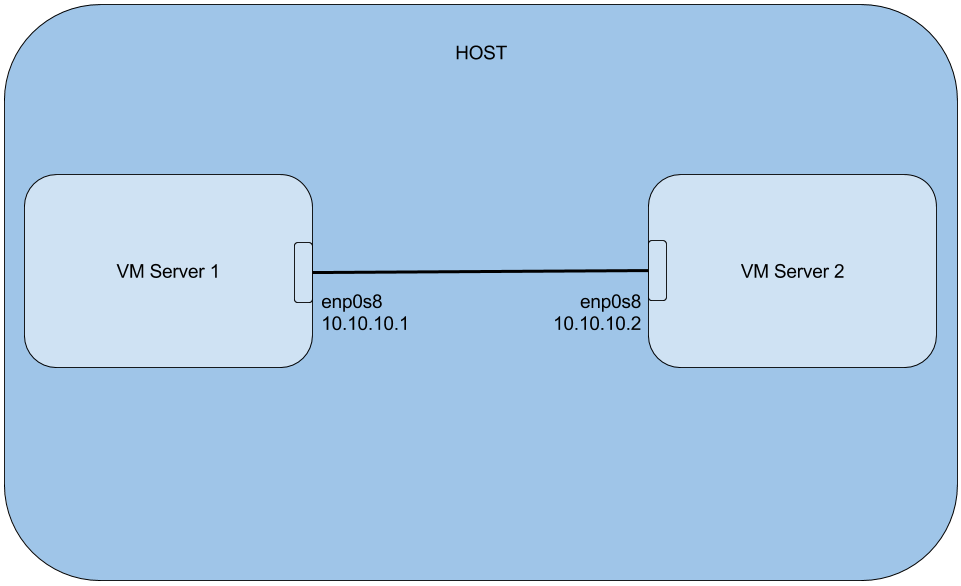
\includegraphics[width=5.5cm]{../tex/figure/vmenv}
      \caption{Overview of Virtual Lab}
      \label{fig:vmenv}
    \end{figure}
    \column{.55\textwidth} % Right column and width
    \texttt{
      \$ ./send\_receive\_packets.sh
      \\\qquad vm
      \\\qquad ostinato
      \\\qquad 1
      \\\qquad 64
      \\\qquad 10
      \\\qquad ./tmp
    }
  \end{columns}
\end{frame}

\section{The End}
\begin{frame}
  \Huge{\centerline{Thank you \& Questions}}
\end{frame}

%----------------------------------------------------------------------------------------

\end{document}
